\documentclass[a4paper,12pt]{article}
\usepackage[slovene]{babel}
\usepackage[utf8]{inputenc}
\usepackage[T1]{fontenc}
\usepackage{graphicx}
\usepackage{amsthm, amsmath}
\usepackage{amssymb} 
\usepackage{subfigure}
\usepackage{url}
\usepackage{subcaption}
\usepackage{booktabs}
\usepackage[margin=2cm]{geometry}

% Podatki za glavo dokumenta:
% Dinamika demokratskih izborov
% Matej Rojec
% 2.2.2025

\title{Dinamika demokratskih izborov}
\author{Matej Rojec}
\date{2.2.2025}

{\theoremstyle{definition}
\newtheorem{algoritem}{Algoritem}
}

\newcommand{\p}{\mathbb{P}} 

\begin{document}

\maketitle
% Glava dokumenta:
% naslov
% povzetek  
\begin{abstract}
    Esej obravnava Galamov model in njegove dinamike \cite{galam2015stubbornness, galam2016trump, galam2020tipping}. Predstavi osnovni model, njegove razširitve ter poudari njegovo uporabnost pri 
    analizi dinamike mnenj v sistemih, ki jih zaznamujejo pomembni dogodki in predsodki. 
    Analizirane so dinamike modela, razširitve pa naslavljajo njegove omejitve in 
    povečujejo uporabnost. Obravnavan je primer volitev Donalda Trumpa leta 2016, 
    ki ponazarja uporabnost modela.
\end{abstract}
% Ključi za sklic na literaturo: galam2015stubbornness, galam2016trump, galam2020tipping

\section{Uvod}

Galamovi modeli, ki jih je v zadnjih 25 letih razvil Serge Galam, obravnavajo dinamiko mnenj, 
odločanje in demokratično glasovanje v hierarhičnih sistemih. 
Uporabljeni so bili za napoved številnih političnih dogodkov, vključno z zmago skrajne desnice 
v Franciji leta 2000 in predsedniškimi volitvami v ZDA leta 2016. Galamov model temelji na 
kritičnih pragovih v javnem mnenju in ideji, da mnenja sledijo univerzalnim zakonitostim. 
Leta 2016 je Galam objavil študijo, ki je pojasnila nepričakovano zmago Donalda Trumpa na 
republikanskih primarnih volitvah in pravilno napovedala njegovo zmago na predsedniških volitvah, 
kar ni bilo podprto z analizami ali anketami. 
Kljub temu ostaja model le eden izmed mnogih in ni popoln, saj so na politične izide vplivali 
številni dejavniki, kot so volilna udeležba in porazdelitev glasov.

\section{Galam model}

% začetek algoritma
\begin{algoritem}
    Galamov model deluje skozi tri ključne korake, ki se iterativno ponavljajo:   

    \begin{enumerate}
    \item Agenti se naključno razporedijo v skupine velikosti od 1 do največ 5 ali 6.
    
    \item V vsaki skupini se uvede lokalno pravilo večine. Pri izenačenju mnenj se mnenje $A$ posodobi z 
    verjetnostjo $k$, mnenje $B$ pa z verjetnostjo $(1-k)$, kar je odvisno od predsodkov v skupini.
    
    \item Vsi agenti se premešajo in postopek se ponovi.
    \end{enumerate}
\end{algoritem}
% konec algoritma

Po več razpravah, ki transformirajo začetno podporo $p_0$ v $p_n$, model doseže končni čas $T$. 
Kandidat $A$ zmaga, če $p_T > \frac{1}{2}$, sicer zmaga kandidat $B$.
Spremembe podpore $A$ in $B$ se izračunajo kot:
\( p_n := \sum_{r=1}^{L} a_r \p_r(p_{n-1}) \),
kjer je $L$ največja velikost skupine, $a_r$ delež skupin velikosti $r$, $\p_r$ pa verjetnost, 
da skupina s $r$ agenti podpira izbiro $A$.

Verjetnost $\p_r$ je izražena kot:
% začetek enačbe
\begin{equation}
    \label{eq:gl}
    \p_{r}(p_{n-1}) = 
    \begin{cases}
        \sum_{m=\frac{r+1}{2}}^r \binom{r}{m} p_{n-1}^m (1-p_{n-1})^{r-m} & \text{za lihe $r$} \\
        \sum_{m=\frac{r}{2} + 1}^r \binom{r}{m} p_{n-1}^m (1-p_{n-1})^{r-m} + k\cdot \binom{r}{\frac{r}{2}} p_{n-1}^\frac{r}{2} (1-p_{n-1})^\frac{r}{2} & \text{za sode $r$}
    \end{cases}
\end{equation}

% 
    % \sum_{m=\frac{r+1}{2}}^r \binom{r}{m} p_{n-1}^m (1-p_{n-1})^{r-m} 
    % za lihe $r$,
    % \sum_{m=\frac{r}{2} + 1}^r \binom{r}{m} p_{n-1}^m (1-p_{n-1})^{r-m} + k\cdot \binom{r}{\frac{r}{2}} p_{n-1}^\frac{r}{2} (1-p_{n-1})^\frac{r}{2}
    % za sode $r$.
% konec enačbe

Glej enačbo \eqref{eq:gl}.

Na kratko premislimo primer, ko je $r$ sodo število. Za podporo izbiri $A$ mora vsaj $\frac{r}{2} + 1$ 
agentov podpreti mnenje $A$, kar zagotavlja večinsko glasovanje. Lahko pa pride tudi do izenačenja 
z $\frac{r}{2}$ agenti za mnenje $A$, pri čemer se izid reši v prid $A$ z verjetnostjo $k$. 

Za dodatno analizo je na grafih \ref{fig:r3} in \ref{fig:r4} prikazana verjetnost $p_n$ 
kot funkcija prejšnje verjetnosti $p_{n-1}$ za različne vrednosti $r$ pri $k=1$.

\begin{figure}[ht!]
    \centering
    \subfigure[Trenutna verjetnost $p_n$ kot funkcija prejšnje verjetnosti $p_{n-1}$ za $k = 1$ in $r = 3$ v intervalu $p_{n-1} \in (0, 1)$.]{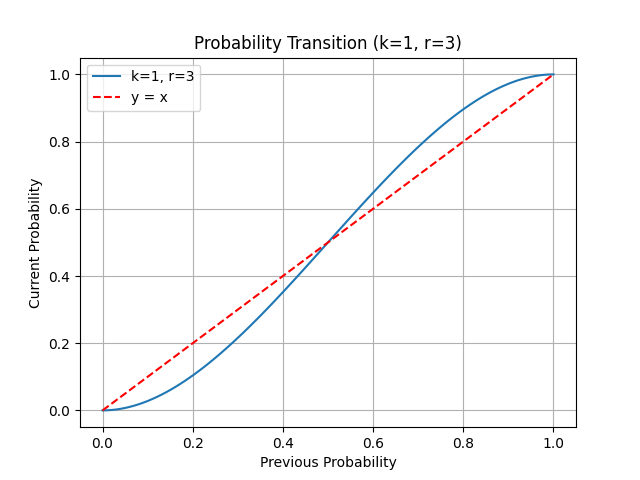
\includegraphics[width=0.4\textwidth]{r3.png}, \label{fig:r3}}, 
    % Slika 1
    % Napis: Trenutna verjetnost $p_n$ kot funkcija prejšnje verjetnosti $p_{n-1}$ za $k = 1$ in $r = 3$ v intervalu $p_{n-1} \in (0, 1)$.
    % Datoteka: r3.png
    % Oznaka: fig:r3
    \subfigure[Trenutna verjetnost $p_n$ kot funkcija prejšnje verjetnosti $p_{n-1}$ za $k = 1$ in $r = 4$ v intervalu $p_{n-1} \in (0, 1)$.]{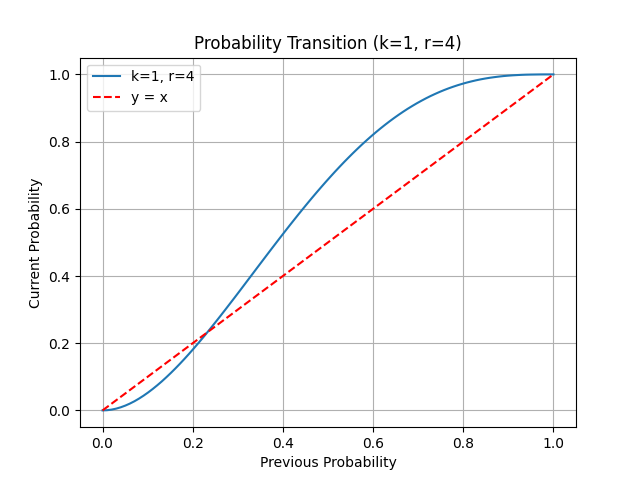
\includegraphics[width=0.4\textwidth]{r4.png}, \label{fig:r4}},
    % Slika 2
    % Napis: Trenutna verjetnost $p_n$ kot funkcija prejšnje verjetnosti $p_{n-1}$ za $k = 1$ in $r = 4$ v intervalu $p_{n-1} \in (0, 1)$.
    % Datoteka: r4.png
    % Oznaka: fig:r4

\end{figure}

% Literatura
\bibliographystyle{plain}
\bibliography{viri.bib} 

\end{document}